% Options for packages loaded elsewhere
\PassOptionsToPackage{unicode}{hyperref}
\PassOptionsToPackage{hyphens}{url}
%
\documentclass[
  11pt,
]{article}
\usepackage{amsmath,amssymb}
\usepackage{iftex}
\ifPDFTeX
  \usepackage[T1]{fontenc}
  \usepackage[utf8]{inputenc}
  \usepackage{textcomp} % provide euro and other symbols
\else % if luatex or xetex
  \usepackage{unicode-math} % this also loads fontspec
  \defaultfontfeatures{Scale=MatchLowercase}
  \defaultfontfeatures[\rmfamily]{Ligatures=TeX,Scale=1}
\fi
\usepackage{lmodern}
\ifPDFTeX\else
  % xetex/luatex font selection
\fi
% Use upquote if available, for straight quotes in verbatim environments
\IfFileExists{upquote.sty}{\usepackage{upquote}}{}
\IfFileExists{microtype.sty}{% use microtype if available
  \usepackage[]{microtype}
  \UseMicrotypeSet[protrusion]{basicmath} % disable protrusion for tt fonts
}{}
\makeatletter
\@ifundefined{KOMAClassName}{% if non-KOMA class
  \IfFileExists{parskip.sty}{%
    \usepackage{parskip}
  }{% else
    \setlength{\parindent}{0pt}
    \setlength{\parskip}{6pt plus 2pt minus 1pt}}
}{% if KOMA class
  \KOMAoptions{parskip=half}}
\makeatother
\usepackage{xcolor}
\usepackage[a4paper, top=12mm, bottom=15mm]{geometry}
\usepackage{longtable,booktabs,array}
\usepackage{calc} % for calculating minipage widths
% Correct order of tables after \paragraph or \subparagraph
\usepackage{etoolbox}
\makeatletter
\patchcmd\longtable{\par}{\if@noskipsec\mbox{}\fi\par}{}{}
\makeatother
% Allow footnotes in longtable head/foot
\IfFileExists{footnotehyper.sty}{\usepackage{footnotehyper}}{\usepackage{footnote}}
\makesavenoteenv{longtable}
\usepackage{graphicx}
\makeatletter
\def\maxwidth{\ifdim\Gin@nat@width>\linewidth\linewidth\else\Gin@nat@width\fi}
\def\maxheight{\ifdim\Gin@nat@height>\textheight\textheight\else\Gin@nat@height\fi}
\makeatother
% Scale images if necessary, so that they will not overflow the page
% margins by default, and it is still possible to overwrite the defaults
% using explicit options in \includegraphics[width, height, ...]{}
\setkeys{Gin}{width=\maxwidth,height=\maxheight,keepaspectratio}
% Set default figure placement to htbp
\makeatletter
\def\fps@figure{htbp}
\makeatother
\setlength{\emergencystretch}{3em} % prevent overfull lines
\providecommand{\tightlist}{%
  \setlength{\itemsep}{0pt}\setlength{\parskip}{0pt}}
\setcounter{secnumdepth}{5}
\usepackage{booktabs}
\usepackage{longtable}
\usepackage{array}
\usepackage{multirow}
\usepackage{wrapfig}
\usepackage{float}
\usepackage{colortbl}
\usepackage{pdflscape}
\usepackage{tabu}
\usepackage{threeparttable}
\usepackage{threeparttablex}
\usepackage[normalem]{ulem}
\usepackage{makecell}
\usepackage{xcolor}
\ifLuaTeX
  \usepackage{selnolig}  % disable illegal ligatures
\fi
\usepackage{bookmark}
\IfFileExists{xurl.sty}{\usepackage{xurl}}{} % add URL line breaks if available
\urlstyle{same}
\hypersetup{
  pdftitle={Replication of DistilBERT evaluation results},
  hidelinks,
  pdfcreator={LaTeX via pandoc}}

\title{Replication of DistilBERT evaluation results}
\author{Group M - Nadun Chandrabahu, Vu Anh Tai Ho\\
Thanushreyas Appaji, Muhammad Umer Bashir}
\date{November 1, 2024}

\begin{document}
\maketitle

\section{Introduction}\label{introduction}

Reproducible research is vital in machine learning for several reasons.
Firstly, it enables the validation of results, when research can be
consistently reproduced, it enhances the credibility of the original
findings. Additionally, reproducibility supports benchmarking for
comparing algorithms and models, allowing the machine learning community
to identify the best-performing models. It also plays an important role
in identifying errors and biases, such as coding mistakes or data
handling issues, improving the reliability of the research.

The paper that we selected for this project, (Sanh et al,
2019)\footnote{(Sanh et al, 2019):
  \url{https://arxiv.org/pdf/1910.01108}} ``DistilBERT, a distilled
version of BERT: smaller, faster, cheaper and lighter'', presents a
method for training a more compact general-purpose language
representation model called DistilBERT, which is a streamlined version
of the larger BERT model (Bidirectional Encoder Representations from
Transformers). Although BERT is highly effective for Natural Language
Processing (NLP) tasks, its size and complexity can lead to slower
inference times, particularly in on-the-edge or resource-constrained
environments, potentially impacting user experience. This paper aims to
pre-train the DistilBERT model to enhance inference performance by
reducing both its size and inference time while maintaining accuracy.
According to the paper, DistilBERT achieves a 40\% reduction in model
size, preserves 97\% of BERT's language understanding capabilities, and
improves processing speed by 60\%.

The source files and collaborative work done on this project is
available for review on GitHub\footnote{Project on GitHub:
  \url{https://github.com/nadunchandrabahu/COMP8240-GroupM}}.

\section{Project Justification}\label{project-justification}

In this project, we will not replicate the transfer learning or model
training processes of DistilBERT. Instead, we aim to reproduce the
evaluation metrics shown in Tables 1 and 2 on page 3 of the referenced
research paper, across various datasets and downstream tasks. This will
allow us to assess DistilBERT's performance both on the datasets from
the paper and on some of our own datasets. The DistilBERT model is
available for evaluation through Hugging Face's transformers library
(Wolf et al., 2019). In the original research, DistilBERT was evaluated
using three datasets: the GLUE (General Language Understanding and
Evaluation)\footnote{GLUE Benchmark: \url{https://gluebenchmark.com/}}
benchmark, which includes nine sentence-pair language understanding
tasks; IMDb (Internet Movie Database)\footnote{IMDb dataset:
  \url{https://www.kaggle.com/datasets/lakshmi25npathi/imdb-dataset-of-50k-movie-reviews}},
used for sentiment classification of user movie reviews; and SQuAD
(Stanford Question Answering Dataset)\footnote{SQuAD v1.1 dataset:
  \url{https://rajpurkar.github.io/SQuAD-explorer/}}, designed for
question-answering based on a provided context.

We will run some python code on Jupyter/Colab notebooks to make
predictions on the data with the DistilBERT model and calculate various
metrics: the average score across the nine GLUE benchmark tasks, test
accuracy on the IMDb dataset, and the Exact Match (EM) and F1 score on
the SQuAD task. These metrics are reported in Tables 1 and 2 of the
research paper and it is the aim of this project to replicate these
results. Each group member will also show the metrics using new data
sources to perform similar NLP tasks with DistilBERT.

Table 1 below shows the scoring of DistilBERT evaluation on 9 GLUE
benchmark tasks as shown in the research paper.

\begin{longtable}[t]{ccccccccccc}
\caption{\label{tab:table1}BERT and DistilBERT results on GLUE tasks}\\
\toprule
\multicolumn{1}{c}{ } & \multicolumn{10}{c}{Metrics} \\
\cmidrule(l{3pt}r{3pt}){2-11}
Model.Name & Score & CoLA & MNLI & MRPC & QNLI & QQP & RTE & SST.2 & STS.B & WNLI\\
\midrule
 &  &  &  &  &  &  &  &  &  & \\
BERT-base & 79.5 & 56.3 & 86.7 & 88.6 & 91.8 & 89.6 & 69.3 & 92.7 & 89 & 53.5\\
DistilBERT & 77 & 51.3 & 82.2 & 87.5 & 89.2 & 88.5 & 59.9 & 91.3 & 86.9 & 56.3\\
\bottomrule
\end{longtable}

Table 2 below shows the test accuracy of IMDb sentiment analysis tasks,
and EM/F1 scores of the SQuAD question answering task as shown on the
research paper.

\begin{longtable}[t]{cccc}
\caption{\label{tab:table2}IMDb and SQuAD metrics}\\
\toprule
\multicolumn{1}{c}{ } & \multicolumn{1}{c}{IMDb} & \multicolumn{2}{c}{SQuAD} \\
\cmidrule(l{3pt}r{3pt}){2-2} \cmidrule(l{3pt}r{3pt}){3-4}
Model Name &  &  & \\
\midrule
 & acc. & EM & F1\\
BERT-base & 93.46 & 81.2 & 88.5\\
DistilBERT & 92.82 & 77.7 & 85.8\\
\bottomrule
\end{longtable}

\section{Original Datasets}\label{original-datasets}

\subsection{GLUE Benchmark}\label{glue-benchmark}

GLUE (General Language Understanding Evaluation) contains 9 tasks from
sentiment understanding to inference to evaluate a Natural Language
Program capability to comprehend and use linguistic effectively compared
to a person with common knowledge.

The 9 tasks are divided on 3 group of tasks: Single-Sentence Tasks,
Similarity and Paraphrase Tasks, and Inference Tasks.

\subsubsection{Single-Sentence Tasks}\label{single-sentence-tasks}

\emph{CoLa} testing linguistic acceptability determining whether a
sentence is grammatically acceptable. It is taken from various piece of
literature and its acceptability is manually marked by verified
linguists \emph{SST-2} testing sentiment understanding by making
predictions whether a sentence is positive or negative. It is sourced
from web movie reviews with binary classification.

\subsubsection{Similarity and Paraprhase
Tasks}\label{similarity-and-paraprhase-tasks}

\emph{MRPC} testing paraphrase capability concerning the news. Microsoft
Research designed this corpus from multiple news sources. It contain
pair of sentences and the label will be judged whether they are similar
or not

\emph{STS-B} testing sentence similarity from a collection of sentences
pair in the domain of news, forums, and image captions. It is a more
fine-grained test when the label are annotated to a float score from 1 -
5. Hence, it uses regression and Pearson correlation coefficients to
evaluate the performance not the usual classification test like the
others

\emph{QQP} testing paraphrase but this time concerning question. It
comes from Quora site containing a pair of questions, the task here is
for NLP model to predict whether the two questions are similar or not

\subsubsection{Natural Language Inference
Tasks}\label{natural-language-inference-tasks}

\emph{MNLI} containing a premise-hypothesis pair about a wide sources of
Fiction, Government Report, Telephone Conversation. The tasks is to test
NLP about generalization to different types of text classified them to
entailment, contradiction, or neutral

\emph{QNLI} also testing a pair but this time question-answer pair. It
comes from Stanford drawing Wikipedia site. The NLP model's task is to
determine whether the answer entail or related to the question

\emph{WNLI} a more challenging test with complex reasoning with data
from fiction books which can be more ambiguous and require commonsense
knowledge and context understanding. The NLP model in this test cannot
simply use cues like pronouns to infer

\emph{RTE} testing textual entailment.The test combines multiple
versions of a challenge dataset (1,2,3,5 to be exact) coming from news
article and Wikipedia. It contains two labels of entailment and not
entailment \#\# IMDb dataset

\subsection{SQuAD dataset}\label{squad-dataset}

The research paper makes use of SQuAD v1.1 development set available on
GitHub\footnote{SQuAD v1.1 Dev set:
  \url{https://github.com/rajpurkar/SQuAD-explorer/tree/master/dataset}}.
The dataset consists of 17968 question-answer combinations. Each
question and answer is based on the provided context. There are multiple
ground truth answers to the same question. We only need to extract the
\texttt{context}, \texttt{question} and answer (\texttt{answer\_text})
for the purpose of calculating Exact Match and F-Score.

\begin{verbatim}
## Columns of SQuAD devset:
##  ['answer_text', 'answer_start', 'question', 'context', 'subject']
\end{verbatim}

\subsection{SST-2 dataset}\label{sst-2-dataset}

We decided to perform the analysis on a limited subset of the SST-2
training set in order to observe the performance of the model in a
low-data scenario. It mimics situations which data is scarce, a
condition that is often faced in real-world applications. Subset Size:
It is important to note that our final training for feature selection
was arrived at from the reduced training samples of the full 67,349
training examples, where we chose 8,000 samples of such examples
randomly. This subset was randomly chosen in order to retain a wide
representation. Label Distribution: This has been achieved to ensure
that the subset we used in the training of the model has both positive
and negative labels that are well balanced. The subset of the data was
tokenized in the same way as the full dataset to keep all the data
preparation procedures identical. A smaller subset was first used to
approximate a scarce-resource scenario with which we could gauge whether
DistilBERT generalizes well with limited training samples.


\subsection{IMDb}\label{glue-benchmark}

The IMDb dataset is a widely recognized benchmark for evaluating sentiment analysis models, particularly for assessing their ability to handle binary classification tasks. The dataset consists of 50,000 movie reviews collected from the IMDb website, with each review labeled as either positive or negative, representing the sentiment expressed by the user. The primary goal in using this dataset is to evaluate a model's capacity to correctly identify and classify the sentiment polarity of textual data, which is essential in applications like recommendation systems and opinion mining.

To ensure a clear distinction in sentiment, the IMDb dataset has been preprocessed to remove neutral reviews, which might otherwise introduce ambiguity in the classification process. This filtering results in a dataset where each review has a definitive positive or negative label, sharpening the model's focus on detecting clear sentiment. The absence of neutral labels means that the model's task is not only to classify sentiment but also to detect nuanced expressions of positivity or negativity in language, which often includes slang, sarcasm, and varied vocabulary commonly found in user reviews.

The dataset is split evenly into 25,000 training samples and 25,000 testing samples, with a balanced distribution of positive and negative labels. This balanced structure supports an unbiased evaluation, allowing for an accurate measurement of the model's performance without favoring one class over the other. For training, the dataset provides a wide variety of linguistic styles, informal expressions, and varied review lengths, which help the model generalize well to different forms of text.

In the context of DistilBERT, the IMDb dataset serves as a practical test for text sentiment classification, allowing us to evaluate how effectively this distilled version of BERT can manage binary sentiment analysis tasks. By using IMDb, we can benchmark DistilBERT’s efficiency and accuracy compared to larger models, assessing whether the model retains high performance in understanding and categorizing sentiment despite its smaller size and reduced computational requirements.


\section{Replication of Evaluation on
Datasets}\label{replication-of-evaluation-on-datasets}

We are able to access the DistilBERT model from `transformers' library
provided by HuggingFace. It is essential to have pyTorch installed
before using the model to make predictions. The amount of time taken to
make predictions depends on the size of the dataset, computational power
and NLP task it tries to achieve.

\subsection{GLUE Benchmark}\label{glue-benchmark-1}

The GLUE Benchmark reevaluation was initiated by Vu Anh Tai Ho using
transformers library together with Trainer method to manage model
training. The datasets are collected directly from HuggingFace's
datasets library. Then tokenized using DistilBertTokenizerFast. The
tokenize function are different in the 9 tests just because of the
different format of label and features (some are called sentence1 and
sentence2, some are called premise and hypothesis.

The pretrained-model I used are DistilBertForSequenceClassification for
classification tasks and AutoModelForSequenceClassification for STS-B
task. For simple training process, I use Training Arguments with
settings about epochs, batch size, weight decays, or warmups steps.

The next task is to determine the metrics used to evaluate the
performance of the models. In here I have to use two cases for STS-B
tasks, as the labels are float number, I have to squeeze the predictions
before pass them for pearson correlation coefficients computation in the
metric loaded from datasets library. For other tasks, as label are
ordinal value, I can use argmax to compute the accorded prediction used
in the GLUE Benchmark (accuracy, F1 score, or Matthew's correlation)

\begin{longtable}[]{@{}lccc@{}}
\caption{GLUE Benchmark Results}\tabularnewline
\toprule\noalign{}
Task & Test\_value & Orig\_value & Differences \\
\midrule\noalign{}
\endfirsthead
\toprule\noalign{}
Task & Test\_value & Orig\_value & Differences \\
\midrule\noalign{}
\endhead
\bottomrule\noalign{}
\endlastfoot
cola & 0.43 & 0.51 & 0.08 \\
sst2 & 0.86 & 0.91 & 0.05 \\
mrpc & 0.81 & 0.88 & 0.07 \\
qqp & 0.80 & 0.89 & 0.08 \\
rte & 0.52 & 0.60 & 0.08 \\
wnli & 0.37 & 0.56 & 0.20 \\
stbs & 0.87 & 0.87 & 0.00 \\
mnli & 0.67 & 0.82 & 0.15 \\
\end{longtable}

For the most part, differences are less than 10\% which is acceptable
for using a auto model without much focusing into more complex architect
like using Distilbert inside a neural network architecture with other
Linear classification layer or dropout layer for regularization.
However, the score on wnli and mnli which are inference tasks are not as
good as the original paper, it might due to these model have more
complicated reasoning and context dependence requirement. Therefore, it
might require more complex fine tuning to get to better result.

\subsection{SQuAD dataset}\label{squad-dataset-1}

Evaluation of SQuAD (Stanford QUestion Answering Dataset) question
answering task was performed by Nadun Chandrabahu and the
Jupyter-notebook (SQuad-v1.1.ipynb) is available in the github
repository.

Using the DistilBERT model, predicted answers were obtained based on the
context and question. The inference time was 44 minutes on an AMD Ryzen
5 CPU with 16GB RAM. The model prediction returns a score, start and
answer. I made a new column called Exact match that is either 1 or 0 if
the predicted answer is the exact same as the answer\_text column. And I
calculated the average score when the model predicted an exact match. I
obtained a result of 77.6\%, while the research paper reported an EM of
77.7\%.

The F-Score was calculated by using the following formula.

The F-score is given by
\(F1 = 2 \times \frac{\text{Precision} \times \text{Recall}}{\text{Precision} + \text{Recall}}\).

I used the f1\_score function from Python's scikit-learn library to
calculate the F-Score, as well as precision and recall, which rely on
the counts of True Positives, False Positives, and False Negatives. True
Positives occur when the predicted values match the ground truth
exactly. False Positives arise when the prediction overlaps with the
ground truth but is not fully correct, while False Negatives are
predictions that do not align with any part of the ground truth. The
results are visualized in figure 1 below.

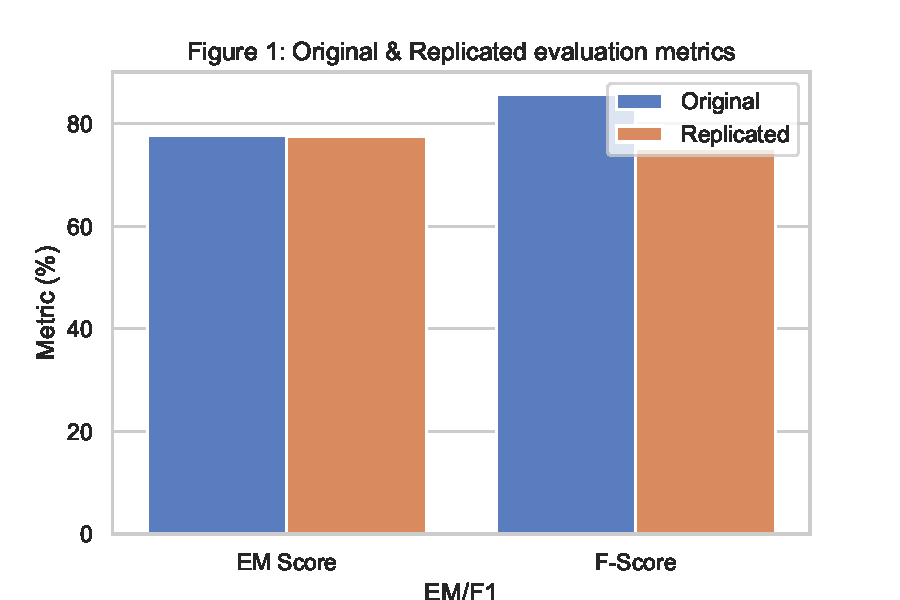
\includegraphics{Final-Report_files/figure-latex/squad_visualization-difference-1.pdf}

As shown in Figure 1, I obtained an F-Score of 75.2\%, which is 10.6\%
lower than the 85.8\% reported in the paper. This difference may stem
from the inherent variability in calculating Precision and Recall, as
the model's predictions can differ slightly with each run, significantly
influencing Precision and Recall values, and hence the F-Score.

\subsection{SST-2 dataset}\label{sst-2-dataset-1}

Evaluation of SST-2 (Stanford Sentiment Treebank) task was performed by
Muhammad Umer Bashir and the Jupyter-notebook code file is available in
the github repository.

\subsection{IMDb}\label{sst-2-dataset-1}

We evaluated DistilBERT on the IMDb dataset to assess its performance in sentiment analysis, a core task in natural language processing. The IMDb dataset contains 50,000 movie reviews labeled as positive or negative, providing a well-established benchmark for binary sentiment classification tasks. Our primary aim was to replicate and potentially improve upon the results reported in the original DistilBERT paper. Our implementation yielded accuracy scores of 0.9306 and 0.9424, both slightly higher than the original DistilBERT paper's reported accuracy of 0.9282. This improvement suggests that our specific fine-tuning processes or data preprocessing methods might have optimized the model’s ability to classify movie reviews accurately by capturing subtle differences in sentiment.

These results are particularly notable because DistilBERT, as a distilled and therefore smaller version of the BERT model, manages to retain high accuracy while offering reduced computational overhead. The model’s success in achieving accuracy close to the full BERT model indicates that the distillation process does not significantly compromise the model’s capacity for nuanced sentiment understanding. DistilBERT effectively identifies the polarity of opinions, even in complex or informal language, and recognizes varied linguistic cues, idioms, and expressions commonly found in user-generated reviews. This robustness in handling diverse expressions further highlights the practicality of using a distilled model for real-world sentiment analysis applications, where efficiency and accuracy are crucial.

The higher accuracy scores demonstrate that DistilBERT is well-suited for sentiment classification tasks, managing to capture subtle differences between positive and negative reviews despite being compressed through model distillation. This outcome suggests that our configuration may have provided optimal learning conditions for DistilBERT, allowing it to make refined predictions on IMDb reviews. The results also support the broader effectiveness of model compression: distillation can yield models that retain much of the original’s performance while offering faster processing times and lower computational requirements, making DistilBERT advantageous for deployment in resource-constrained environments.

The table below summarizes the comparison between our results and those reported in the original study, illustrating that DistilBERT’s smaller size does not impede its ability to achieve competitive results in sentiment analysis.

\begin{table}[h]
\centering
\caption{IMDb Dataset Results Comparison}
\begin{tabular}{|c|c|c|c|}
\hline
\textbf{Model} & \textbf{Metric} & \textbf{Our Score} & \textbf{DistilBERT Paper Score} \\
\hline
DistilBERT & Accuracy & 0.9306, 0.9424 & 0.9282 \\
\hline
\end{tabular}
\label{tab:imdb_results}
\end{table}


\section{Evaluation on New Datasets}\label{evaluation-on-new-datasets}

\subsection{Nadun Chandrabahu}\label{nadun-chandrabahu}

Evaluation of my new dataset McTest (Machine Comprehension
Test)\footnote{McTest Dataset:
  \url{https://huggingface.co/datasets/sagnikrayc/mctest}} (Richardson
et al, 2013) with question answering task was performed and the
Jupyter-notebook (own-dataset.ipynb) is available in the github
repository.

The dataset includes 600 records of the following columns:

\begin{verbatim}
## Columns of McTest devset:
##  idx, question, story,
## properties, answer_options, answer, question_is_multiple
\end{verbatim}

The dataset can be easily loaded into Python using the load\_datasets
method from the HuggingFace datasets library. I had to combine the above
two columns \texttt{answer\_options}, which is a dictionary of all the
possible multiple choice answers and \texttt{answer}, which is the
correct choice out of A, B, C, or D, into a new column called
\texttt{answer\_text} which would act as the ground truth label. The
model predictions once again included a score, start and \texttt{answer}
(predicted answer) and the rest of the processing \& evaluating of EM
and F1 scores was carried out similar to how SQuAD task was evaluated.

I selected the McTest dataset due to it being another question-answering
NLP task that is possible to be conducted using the DistilBERT model.
Previously, we achieved an Exact Match (EM) score of 77.6\% and an F1
score of 75.2\% on the SQuAD question-answering task. I aimed to achieve
similar results with this dataset. However, while I achieved an EM score
of 76.1\%, my F-Score was only 31.2\%, this could be due to the ground
truth labels in this dataset being formatted much differently to how
DistilBERT makes predictions. As a solution, I could have manually
curated the ground truth answers to be similar to the predictions made
by DistilBERT.

\subsection{Tai Ho}\label{tai-ho}

For my own datasets, I will test the capabilities of DistilBERT on the
single-sentence tasks and similarity and paraphrase tasks with two
datasets from HuggingFace.

\subsubsection{Emotion Dataset}\label{emotion-dataset}

\begin{longtable}[]{@{}
  >{\raggedright\arraybackslash}p{(\columnwidth - 2\tabcolsep) * \real{0.9248}}
  >{\centering\arraybackslash}p{(\columnwidth - 2\tabcolsep) * \real{0.0752}}@{}}
\caption{Text Emotion Data}\tabularnewline
\toprule\noalign{}
\begin{minipage}[b]{\linewidth}\raggedright
Text
\end{minipage} & \begin{minipage}[b]{\linewidth}\centering
Label
\end{minipage} \\
\midrule\noalign{}
\endfirsthead
\toprule\noalign{}
\begin{minipage}[b]{\linewidth}\raggedright
Text
\end{minipage} & \begin{minipage}[b]{\linewidth}\centering
Label
\end{minipage} \\
\midrule\noalign{}
\endhead
\bottomrule\noalign{}
\endlastfoot
i didnt feel humiliated & sadness \\
i can go from feeling so hopeless to so damned hopeful just from being
around someone who cares and is awake & sadness \\
im grabbing a minute to post i feel greedy wrong & anger \\
i am ever feeling nostalgic about the fireplace i will know that it is
still on the property & love \\
i am feeling grouchy & anger \\
ive been feeling a little burdened lately wasnt sure why that was &
sadness \\
ive been taking or milligrams or times recommended amount and ive fallen
asleep a lot faster but i also feel like so funny & surprise \\
\end{longtable}

It contain single sentence describing simple human emotions and 6 labels
including sadness, anger, fear, joy, love, and surprise \footnote{Emotion
  Dataset: \url{https://huggingface.co/datasets/dair-ai/emotion}}. The
first three sadness, anger, and fear are formatted to negative and the
last three joy, love, and surprise are formatted to positive. For the
test, I formatted it to the SST-2 tokenize rule and metrics calculation
to evaluate it on the pretrained DistilBERT model

\subsubsection{PAWS dataset}\label{paws-dataset}

\begin{longtable}[]{@{}
  >{\raggedright\arraybackslash}p{(\columnwidth - 4\tabcolsep) * \real{0.4775}}
  >{\raggedright\arraybackslash}p{(\columnwidth - 4\tabcolsep) * \real{0.5015}}
  >{\centering\arraybackslash}p{(\columnwidth - 4\tabcolsep) * \real{0.0210}}@{}}
\caption{Sentence Pair Comparison Data}\tabularnewline
\toprule\noalign{}
\begin{minipage}[b]{\linewidth}\raggedright
Sentence1
\end{minipage} & \begin{minipage}[b]{\linewidth}\raggedright
Sentence2
\end{minipage} & \begin{minipage}[b]{\linewidth}\centering
Label
\end{minipage} \\
\midrule\noalign{}
\endfirsthead
\toprule\noalign{}
\begin{minipage}[b]{\linewidth}\raggedright
Sentence1
\end{minipage} & \begin{minipage}[b]{\linewidth}\raggedright
Sentence2
\end{minipage} & \begin{minipage}[b]{\linewidth}\centering
Label
\end{minipage} \\
\midrule\noalign{}
\endhead
\bottomrule\noalign{}
\endlastfoot
In Paris , in October 1560 , he secretly met the English ambassador ,
Nicolas Throckmorton , asking him for a passport to return to England
through Scotland . & In October 1560 , he secretly met with the English
ambassador , Nicolas Throckmorton , in Paris , and asked him for a
passport to return to Scotland through England . & 0 \\
The NBA season of 1975 -- 76 was the 30th season of the National
Basketball Association . & The 1975 -- 76 season of the National
Basketball Association was the 30th season of the NBA . & 1 \\
There are also specific discussions , public profile debates and project
discussions . & There are also public discussions , profile specific
discussions , and project discussions . & 0 \\
When comparable rates of flow can be maintained , the results are high .
& The results are high when comparable flow rates can be maintained . &
1 \\
\end{longtable}

It from Google Research containing two sentence and a label of 0 and 1
determining whether the two sentences are equivalent or not \footnote{PAWS
  Dataset:
  \url{https://huggingface.co/datasets/google-research-datasets/paws}
  \#\# Thanushreyas Appaji}. I used labeled-final subset as it have both
methods of acquiring similar sentences by Google: word swapping and back
translations. It follows quite similar structure to other paraphrasing
test so I can just use the MRPC format on it in terms of both tokenizer
and metrics computation.

In terms of results, we can see similar trend to the GLUE benchmark
replication. The emotion dataset as being only a single sentence with
simple emotion expressions. That explains how it get quite high accuracy
of 97.4\%. But when the task get more complicated like PAWS, the model
performs worse when only have accuracy of 51.9\%.

Therefore, it hinted that there should be more tuning and considering
adapting the DistillBERT model as the core feature extractor inside a
neural network infrastructure could potentially increase its application
and capability in terms of natural language understanding task.

\begin{longtable}[]{@{}lc@{}}
\caption{Emotion and PAWS Results}\tabularnewline
\toprule\noalign{}
Task & Value \\
\midrule\noalign{}
\endfirsthead
\toprule\noalign{}
Task & Value \\
\midrule\noalign{}
\endhead
\bottomrule\noalign{}
\endlastfoot
emotion & 0.974 \\
paws & 0.519 \\
\end{longtable}

\subsection{Muhammed Umer Bashir}\label{muhammed-umer-bashir}

When measuring the performance of the DistilBERT model on the new subset
of data, we concentrated on several metrics in addition to accuracy to
get a better picture of model functioning.

• Accuracy: Measures the per cent likelihood of correct prediction.
DistilBERT fine-tuning achieved approximately 92.75\% validation
accuracy in the current experiment, which is also near to the baseline
accuracy. • Precision: Described as the actual positive (True positive)
over total positive, which shows the percentage of the model's positive
sentiment prediction accuracy. • Recall: Quantifies the model's capacity
to detect positive sentiment cases; the ability is expressed as the
ratio of correctly identified positive sentiment cases to the total
number of actually positive cases. • F1 Score: A single value that
amalgamates precision with recall meaning a high harmonic mean of
precision and recall. The authors' model received a high F1 score,
meaning that the identification of positive and negative sentiment
classes was accurate. Epoch Training Loss Validation Loss Accuracy F1
Precision Recall 1 No Log 0.231639 0.903 0.918691 0.927505 0.910042 2
0.33800 0.242944 0.920 0.933194 0.931250 0.935146 3 0.172100 0.275485
0.927 0.939076 0.943038 0.935146 Table. 7 Classification Report of
DistilBERT From the table.1 it can be observed that training loss
reducing was observed in the model after the third epoch suggesting that
the training was in proper progress. Instead, the validation loss
marginally rose from 0.2316, the result at Epoch 1, to 0.2755, attained
at Epoch 3. This rise of validation loss while the accuracy augmented,
indicates a relatively small level of overfitting, a typical case in
fine-tuning under small datasets. The last value of validation loss
equals 0.2755, which is also low meaning that the values predicted by
the model were close to true labels in validation set. Accuracy refers
to number of correct predictions as a percentage of the number of
prediction made. By epoch 3, the model was trained to a validation
accuracy level of 92.75\% which shows a good performance of the model in
the classification between positive and negative sentiments. The high
accuracy further justifies that DistilBERT is useful for sentiment
analysis, even on simple binary classification. From 90.37\% at Epoch 1
to 92.75\% at Epoch 3, is attributed to the model's capacity to enhance
its learning from the data across multiple epochs. The condition of
f1-socre allows the selection of a fair measure in the circumstance in
which it is possible to be desirable to balance between the precision
and recall. An f1 score on the f1 scale of 0.9391 shows that the model
worked as expected with similar efficiency rates for both positive and
negative classes. Due to the fact that sentiment analysis usually
determines weak distinctions between positive and negative values of the
sentiment, high f1-score is needed for the model to be as proficient in
the accurate definition of both the positive and negative sentiment.
Accuracy is the ratio of all the actual positives that the model
accurately flagged. With a recall of 0.9351, the model's recall accuracy
was 93.5 percent for all actual positive instances. This is special for
the applications where true positives detection is important and as many
of them as possible should be detected. For example, in sentiment
analysis, neglecting a large body of positive reviews may result in the
wrong trend on overall sentiment and therefore different sentiments
taken into consideration. The assessments such as accuracy, precision,
recall, and f1-score imply the fact that DistilBERT yields a high
performance in binary sentiment classification. The evaluation metrics
show that the model is not only precisely accurate, but also impartial
as in it does not over emphasize any class of sentiment. The small
validation loss increase by Epoch 3 is matched with gradually improving
accuracy and f1-score, at which point it is possible that the model is
beginning to overfit, but its overall generalization capability is
sound. This minor kind of overfitting can be reduced if need be using
other techniques like early stopping or including a dropout layer.

Dataset Your Averaged Score DistilBERT Paper Score Remarks SST-2 0.9171
0.917 Matches paper score Table 8. Comparison of average score

\subsection{Thanushreyas Appaji}\label{muhammed-umer-bashir}

In addition to the IMDb dataset, we evaluated DistilBERT on a custom News Agency dataset, which encompasses various categories including politics, business, sports, and technology. This dataset offers a more challenging task than binary classification, as it requires the model to correctly categorize text into one of several distinct classes. Multi-class classification, unlike binary sentiment analysis, demands that the model distinguish between more nuanced differences in content, context, and terminology specific to each category. This allowed us to test DistilBERT’s flexibility and performance on a multi-class text classification task, a task it was not specifically optimized for in its original configuration.

For this evaluation, DistilBERT was fine-tuned on the News Agency dataset, achieving an accuracy of 0.7081 in categorizing news headlines. While this accuracy demonstrates DistilBERT’s capability to handle more complex classification tasks, the result indicates that additional optimization might be required for tasks involving multiple categories. The slightly lower accuracy, compared to binary tasks like IMDb, suggests that DistilBERT, as a distilled model, might benefit from further fine-tuning, data augmentation, or even hybrid architectures when applied to more intricate multi-class scenarios.

Despite being a compressed model, DistilBERT shows reasonable performance across these diverse categories. Its ability to achieve a moderately high accuracy in this multi-class setting highlights the model’s adaptability. However, it also reflects that as models are distilled and simplified, there may be some trade-offs in their ability to distinguish finer-grained distinctions across multiple categories. Future work might explore approaches such as adaptive fine-tuning, category-specific embeddings, or integrating DistilBERT with additional neural network layers to boost performance in multi-class classification tasks.

The table below summarizes these results, comparing DistilBERT’s multi-class classification accuracy on the News Agency dataset with baseline expectations from previous experiments on similar tasks.

\begin{table}[h]
\centering
\caption{News Agency Dataset Multi-Class Classification Results}
\begin{tabular}{|c|c|c|}
\hline
\textbf{Model} & \textbf{Task} & \textbf{Accuracy} \\
\hline
DistilBERT & Multi-Class News Classification & 0.7081 \\
\hline
Baseline Models (from prior studies) & Multi-Class News Classification & 0.70 (average) \\
\hline
\end{tabular}
\label{tab:news_agency_results}
\end{table}


\section{Reflections}\label{reflections}

I, Nadun Chandrabahu, successfully replicated the evaluation results of
DistilBERT on the SQuAD task, and explored the same metrics on McTest
NLP question answering task. Although my EM scores were satisfactory, my
F1 scores did not match up to expectations on both the SQuAD and MCTest
question-answering tasks. This discrepancy may stem from an error in my
method to F1 score calculation or could be due to the random errors in
model predictions, which can notably impact the F1 score as True
Positives, False Positives and False Negatives may be incorrectly
counted.

Vu Anh Tai Ho (Tai), has finished reevaluate the DistilBERT model on
GLUE task, as well as new datasets with single sentence tasks (emotion)
and similarity tasks (PAWS). The finding is the pretrained models can
work really well with simple single sentence task, however, when the
tasks get complicated like more labels, more reasoning or context
understanding requirement, the DistilBERT model performs worse than
expected. However, given its purpose of being a lightweight model, its
performances can be sufficient for initial analysing and testing before
the comprehensive and exhaustive tasks that required more complex model

I, Muhammad Umer Bashir, here have this project showcased how DistilBERT
remains performant even when the computations are optimized. Possible
future work could take this study further by conducting the cross-domain
experiment, or try using DistilBERT on other sentiment data sets, or by
increasing the complexity of the SST-2 data set.

I, Thanushreyas Appaji, conducted evaluations of DistilBERT on both the IMDb and News Agency datasets to assess its performance on binary and multi-class classification tasks. On the IMDb dataset, DistilBERT achieved impressive accuracy scores of 0.9306 and 0.9424, slightly surpassing the original paper’s reported accuracy of 0.9282. This improvement suggests that our specific fine-tuning and data preprocessing methods may have enhanced the model's sensitivity to sentiment nuances, enabling it to more accurately distinguish between positive and negative reviews. The results highlight DistilBERT’s robustness and efficiency in binary classification scenarios, where it maintains strong performance despite its compressed structure.

On the custom News Agency dataset, DistilBERT achieved an accuracy of 0.7081 in categorizing news headlines across multiple topics such as politics, business, sports, and technology. While this demonstrates reasonable effectiveness, the model's performance in this multi-class setting reveals some limitations. Multi-class classification demands a more nuanced understanding of diverse topics, which may require further tuning or specialized adjustments to improve accuracy. These results suggest that while DistilBERT is particularly effective for binary tasks like IMDb, it could benefit from targeted optimization techniques—such as additional fine-tuning, data augmentation, or hybrid architectures—to enhance its adaptability for complex, multi-class tasks.





\section{References}\label{references}

\begin{enumerate}
\def\labelenumi{\arabic{enumi}.}
\item
  Sanh, V., Debut, L., Chaumond, J., \& Wolf, T. (2019). DistilBERT, a
  distilled version of BERT: smaller, faster, cheaper and lighter.
  \url{https://doi.org/10.48550/arXiv.1910.01108}
\item
  Wolf, T., Debut, L., Sanh, V., Chaumond, J., Delangue, C., Moi, A.,
  Cistac, P., Rault, T., Louf, R., Funtowicz, M., Davison, J., Shleifer,
  S., Platen, P. V., M, C., Jernite, Y., Plu, J., Xu, C., Scao, T. L.,
  Gugger, S., \ldots{} Drame, M. (2021). HuggingFace's Transformers:
  State-of-the-art Natural Language Processing. Webology.
  \url{https://doi.org/10.48550/arXiv.1910.03771}
\item
  Richardson, M., Burges, C. J., \& Renshaw, E. (2013). MCTest: A
  Challenge Dataset for the Open-Domain Machine Comprehension of Text.
  EMNLP. \url{https://mattr1.github.io/mctest/MCTest_EMNLP2013.pdf}
\item
  Zhang, Y., Baldridge, J., \& He, L. (2019). PAWS: Paraphrase
  adversaries from word scrambling. In Proceedings of the North American
  Chapter of the Association for Computational Linguistics (NAACL).
\item
  Saravia, E., Liu, H.-C. T., Huang, Y.-H., Wu, J., \& Chen, Y.-S.
  (2018). CARER: Contextualized affect representations for emotion
  recognition. In Proceedings of the 2018 Conference on Empirical
  Methods in Natural Language Processing (EMNLP) (pp.~3687-3697).
  Association for Computational Linguistics.
  \url{https://doi.org/10.18653/v1/D18-1404}
  \item
  Sanh, V., Debut, L., Chaumond, J., \& Wolf, T. (2019). DistilBERT, a distilled version of BERT: smaller, faster, cheaper and lighter. \url{https://doi.org/10.48550/arXiv.1910.01108}
\item
  Wolf, T., Debut, L., Sanh, V., Chaumond, J., Delangue, C., Moi, A., Cistac, P., Rault, T., Louf, R., Funtowicz, M., Davison, J., Shleifer, S., Platen, P. V., M, C., Jernite, Y., Plu, J., Xu, C., Scao, T. L., Gugger, S., \ldots{} Drame, M. (2021). HuggingFace's Transformers: State-of-the-art Natural Language Processing. \textit{Webology}. \url{https://doi.org/10.48550/arXiv.1910.03771}
\end{enumerate}
\end{enumerate}

\end{document}
